\documentclass{article}

% imports
\usepackage[margin=1in]{geometry}
\usepackage{multirow}
\usepackage{graphicx}
\usepackage{subcaption}
\usepackage{listings}
\usepackage{natbib}
\usepackage{amsmath} % split environment
\usepackage{booktabs} % \toprule, \midrule, and \bottomrule commands,
\usepackage{array} % for \arraybackslash
\usepackage{calc}
\usepackage{tabularx}

% begin document
\begin{document}

% title
\begin{titlepage} % Suppresses displaying the page number on the title page and the subsequent page counts as page 1
	\newcommand{\HRule}{\rule{\linewidth}{0.5mm}} % Defines a new command for horizontal lines, change thickness here
	
	\center % Centre everything on the page
	
	%------------------------------------------------
	%	Headings
	%------------------------------------------------
	
	\textsc{\LARGE IT Univeristy Of Copenhagen}\\[1.5cm] % Main heading such as the name of your university/college
	\textsc{\Large BSc Data Science}\\[0.5cm] % Major heading such as course name
	\textsc{\large Final Thesis}\\[0.5cm] % Minor heading such as course title
	
	%------------------------------------------------
	%	Title
	%------------------------------------------------
	
	\HRule\\[0.4cm]
	{\huge\bfseries Bayesian Modelling for Real-World Revenue Forecasting}\\[0.4cm] % Title of your document
	\HRule\\[1.5cm]
	
	%------------------------------------------------
	%	Author(s)
	%------------------------------------------------
	Louis \textsc{Brandt} \\
	\texttt{locb@itu.dk}
	%------------------------------------------------
	%	Date
	%------------------------------------------------
	
	\vfill\vfill\vfill % Position the date 3/4 down the remaining page
	{\large\today} % Date, change the \today to a set date if you want to be precise
	
	%------------------------------------------------
	%	Logo
	%------------------------------------------------
	%\vfill\vfill
	%\includegraphics[width=0.2\textwidth]{placeholder.jpg}\\[1cm] % Include a department/university logo - this will require the graphicx package
	
	%----------------------------------------------------------------------------------------
	\vfill % Push the date up 1/4 of the remaining page
	
\end{titlepage}
%----------------------------------------------------------------------------------------


% table of contents
\tableofcontents
\newpage

% abstract
% \begin{abstract}
This study investigates using Bayesian models for daily revenue forecasting on
the case study of OLIOLI, a Copenhagen-based poke bowl chain. A comprehensive
assessment of various Bayesian models reveals their predictive strengths and
limitations within a real-world context. The research examines the influence of
weather indicators, such as maximum temperature and total precipitation, on
revenue. In the case study, Bayesian time-series models outperform their linear
regression counterparts, and weather factors are not found to add significant
value in models, treating revenue as a time-series. This challenges expert
assumptions about the causal relationship between weather and revenue. Offering
a thorough evaluation of Bayesian models for revenue prediction, this study
invites further inquiry into the complex relationships between environmental
factors and daily revenue for this case. It provides practical insights for revenue
forecasting for this case study and a critical perspective on Bayesian data
analysis assumptions and implications.
\end{abstract}


% introduction
\section{Introduction}

% ------------------- Introduce Bayes --------------------------

Accurate revenue forecasting plays a pivotal role in the success of businesses,
aiding in efficient resource allocation, planning, and well-informed
decision-making. In this study, we delve into the application of Bayesian
models for predicting daily revenue at Copenhagen based poke bowl chain called
OLIOLI. By comparing the performance of various Bayesian models and evaluating
their usefulness, we aim to provide insights into the advantages and
limitations of these methods in a real-world context, and contribute to the
ongoing research in the field of Bayesian data analysis.
% Intuitive questions: Fixing observed data and updating beliefs about model parameters
Grounded in the principles of Bayes' theorem, Bayesian modeling provides an
alternative to the classic frequentist approach in data analysis and modeling.
Bayesian methods incorporate prior knowledge and facilitate a more intuitive
understanding of uncertainty, which can be particularly useful for tackling
complex real-world challenges.
% Handling uncertainty 
In practice, the prior belief is represented by a probability distribution over
the model parameters, which is updated to a posterior distribution after
observing data. This posterior distribution is then used to make predictions
and inferences about the model parameters. By their nature, probability
distributions are well suited to represent uncertainty 
% Model comparison and selection
% Additionally, the Bayesian method provides a principled framework for the comparison 
% and selection of different models. The best model for a problem is assumed to be 
% the most simple model able to explain the observed data and bayesian comparison methods 
% discussed in this paper provide a way to quantify this simplicity.

% ------------------- Define the problem --------------------------
% Daily revenue prediction
One area where modelling uncertainty is helpful is in revenue prediction and forecasting. 
This paper focuses on a case study to illustrate the application of Bayesian methods
and how the various decisions at steps of processing, modelling and comparison propegate 
to the final model and its predictions.
% Real-world phenomena complexity
When modelling real-world phenomena, the complexity of the problem can make it difficult 
to find a useful model - accurate and interpretable - and is therefore an exciting domain 
to test and evaluate theoretical methods.
% Revenue as a compound of individual human decisions
The revenue of a store is a compound of an immeasurable number individual human
decisions, which makes choosing the relavent, measurable variables of interest
a challenge. 
% Deciding on variables of interest: Expert opinion, domain knowledge, time series analysis
Here, we are guided by experts and their domain knowledge, who
have long been aware of the various temporal factors that influence revenue -
and what daily, weekly, and seasonal patterns mean for the business. The
weather thought to be another source of variablility throughout OLIOLI and it
was this that motivated the study of various weather phenomena on revenue.

% ------------------ Research Questions ----------------------------

In light of these approaches, the research questions that will be addressed in this paper are:

\begin{enumerate}
    \item What is the best performing Bayesian model for predicting daily revenue for OLIOLI with weather data?
    \item What is the optimal data volume for optimal revenue prediction?
    \item What are the assumptions and compromises of different models, and how do they impact the performance and the interpretability of the results?
\end{enumerate}

% ---------- Testing, evaluation, Bayesian comparison ------------

% Using real-world sales data for the case study
% Selection of the optimal model and data for specific problems
% Context-dependent decision-making
To answer these questions, we will test, compare and evaluate multiple Bayesian
models and evaluation metrics, using real-world sales data from OLIOLI. Current
research in the field exists for motivating the deployment of Bayesian models,
with methodologies existing for their evaluation and comparison. Despite this,
the exact process for selecting the optimal model and data for a specific
problem remains unclear and context-dependent.

This paper consists of five further sections. First, background theory is
introduced aimed to provide a foundation of knowledge from which the Bayesian
analysis of the case study can be understood. Second, the case study is
introduced and the data is investigated. Third, the methodology motivates and
describes the models, as well as reflecting on the initial predictive
performance of the various approaches applied to the case study. Fourth, the
results are fully presented, discussed and the Bayesian models are compared.
Finally, the paper is concluded with a summary of the findings and a discussion
of the limitations and future work of the study.

% ------------------ Contributions -------------------------------

% Thorough testing, evaluation, and comparison of different assumptions in Bayesian data analysis
% Focus on revenue prediction for a restaurant chain
% Potential for accurate forecasting, better decision-making, and efficient resource allocation
The contributions of this paper are manifold, providing a comprehensive
testing, evaluation, and comparison of the different assumptions within the
realm of Bayesian data analysis; through the vessel of the mentioned case
study. By investigating the research questions and evaluating the performance
of various Bayesian models, this study aims to not only demonstrate the
potential for accurate forecasting but also emphasise the potential benefit of
informed decision-making and efficient resource allocation in a business
context.
% Hierarchical extension possibilities


% background
\section{Background}

% ------------------- Introduce Bayes --------------------------

\subsection{Bayesian Statistics}

This paper does not aim to serve as a guide to Bayesian statistics, nor an
explicit introduction to the theory. Nonetheless, some background knowledge is
necessary in understanding the theory and assumptions motivated throughout the
paper.

In Bayesian statistics, the foundational interpretation of probability differs
from traditional frequentist statistics. In the more familiar frequentist approach,
probability is defined as the long-run frequency of an event occurring, the
intuition of which can be built with the example of a coin flip. The
probability of a coin landing on heads is assumed to be a fixed but unknown
quantity, and when a coin is flipped 100 times, and 60 of those flips result in
heads, the probability of heads is defined as 0.6. 

In contrast, Bayesian statistics defines probability as a measure of belief and
model parameters - like the true fairness of a coin - are assumed to be random
variables. Our belief about the probability of heads is represented by a prior
distribution, which is updated based on observed data. If a coin is flipped 100
times and heads observed 60 times, this prior belief about the probability of
heads is updated to a posterior distribution that reflects our new
understanding of the coin's behavior, taking into account both the observed
data and our initial belief. This posterior distribution allows us to quantify
our uncertainty about the probability of heads and make predictions - or
inferences - about future coin flips.

\subsubsection{Bayes' Theorem}

The framework for updating beliefs in Bayesian statistics is Bayes' Theorem;
derived from the definition of conditional probability. Bayes' Theorem
describes the probability of an event, based on prior knowledge of conditions 
that might be related to the event, and observed evidence. 
The general form of Bayes' Theorem is given by:
\begin{equation}
  P(A|B) = \frac{P(B|A)P(A)}{P(B)}
\end{equation}
Applications of the Bayesian framework are vast; the belief in any hypothesis can
be logically updated when new evidence is encountered.
\begin{equation}
  P(\text{Hypothesis}|\text{Evidence}) = \frac{P(\text{Evidence}|\text{Hypothesis})P(\text{Hypothesis})}{P(\text{Evidence})}
\end{equation}
In the context of Bayesian modeling, we are interested in updating our beliefs
about the parameters of a model given some observed data.
\begin{equation}
  P(\text{Parameters}|\text{Data}) = \frac{P(\text{Data}|\text{Parameters})P(\text{Parameters})}{P(\text{Data})}
\end{equation}
\begin{table}[h]
\centering
\begin{tabular}{lll}
\toprule
Term & Symbol & Description \\
\midrule
Posterior & $P(\text{Parameters}|\text{Data})$ & Updated belief about the parameters given the data \\
Likelihood & $P(\text{Data}|\text{Parameters})$ & Probability of observing the data given the parameters \\
Prior & $P(\text{Parameters})$ & Initial belief about the parameters before observing the data \\
Evidence & $P(\text{Data})$ & Probability of observing the data \\
\bottomrule
\end{tabular}
\caption{Components of Bayes' theorem in the context of Bayesian modeling.}
\label{tab:bayes_theorem}
\end{table}

\subsubsection{Priors}
Unique to Bayesian statistics is the concept of prior distributions. Priors are
probability distributions that represent the beliefs about the model parameters
before observing any data. \cite{clinical} does a fine job of illustrating the
impact of priors on the posterior distribution, shown in figure
\ref{fig:prior-impact}. 
\begin{figure}
  \begin{center}
    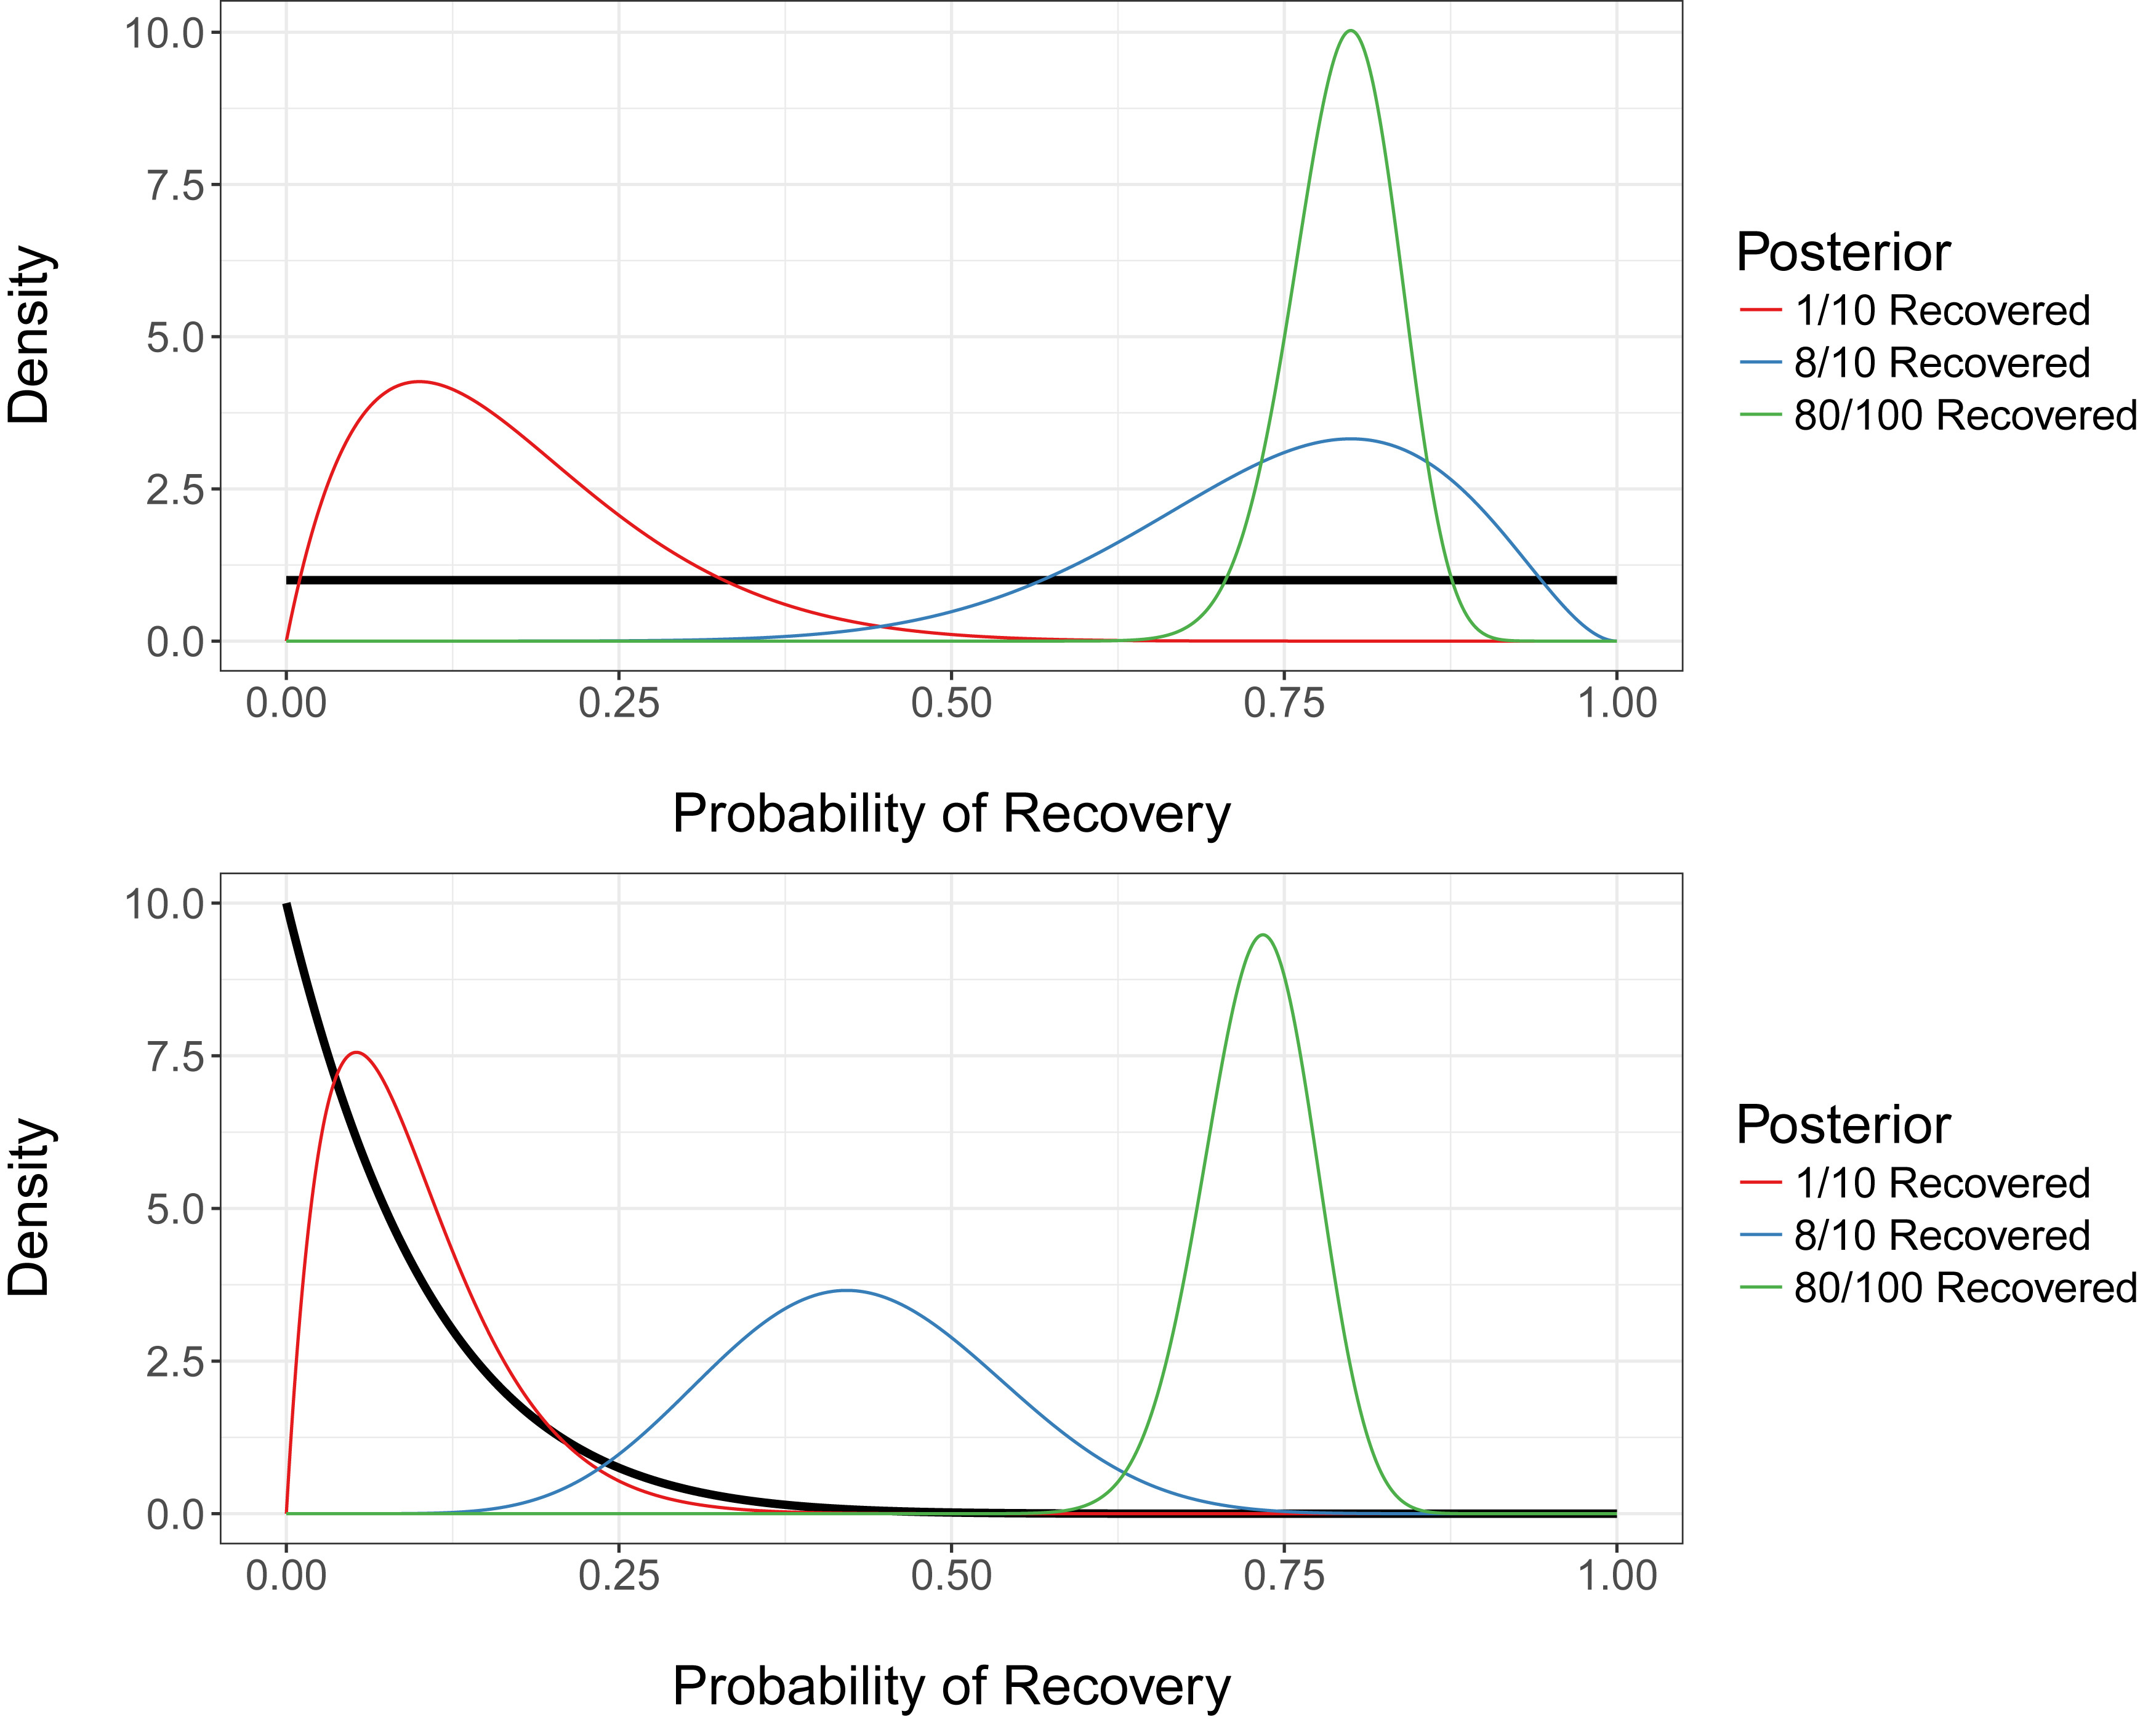
\includegraphics[width=0.5\textwidth]{../imgs/prior-impact.jpg}
  \end{center}
  \caption{Plots demonstrating the impact of different priors and data on posterior distributions. The top figure is for a flat prior distribution and the bottom figure is for an informative prior distribution. Solid black line is the prior distribution, colored lines are the posterior distributions, \cite{clinical}.}
  \label{fig:prior-impact}
\end{figure}
They are often a talking point in the validity of experiments utilising a
Bayesian approach as, while incorporation of prior knowledge can be a key
factor in Bayesian models outperforming other frequentist models, especially
when the amount of data is limited; they can also be seen as a daunting source
of subjectivity.
There are two main philosophies when it comes to selecting priors, objective
and subjective Bayesianism. 

\textbf{Objective Bayesianism} aims to minimise the influence of personal
beliefs on the analysis by using priors that are as non-informative as
possible. Objective priors, often called non-informative or reference priors,
are chosen based on the principle of indifference or maximum entropy, which
tries to represent a state of ignorance about the parameters. The goal is to
allow the data to have the most influence on the posterior distribution. This
approach is often favored when there is limited prior knowledge or when
researchers wish to avoid potential bias from subjective beliefs. However, even
with the best intentions in mind, no prior can be truly non-informative, and
objective priors can still carry some level of subjectivity in their selection.

\textbf{Subjective Bayesianism}, on the other hand, embraces the idea that
personal beliefs and prior knowledge should be incorporated into the analysis.
Subjective priors are chosen based on a researcher's knowledge, expertise, and
beliefs about the parameters of interest. This approach allows for the
integration of existing information and expert opinions, which can result in
more accurate and informative inferences, especially in cases where data are
limited or noisy. Some argue that subjective priors can introduce bias, as they
rely on the researcher's personal beliefs. However, the opposing argument that
scientific research inherently subjective to some degree, and transparency
about the choice of priors, at worst allows for open evaluation and discussion
within the research community.
\cite{clinical} addresses the viewpoint that, on the surface, it might seem
outright wrong that two otherwise identical experiments can yield different
results, simply because different prior beliefs were defined. Baldwin and
Larson show that this argument is mitigated by the fact that subjectivity is
inherent in research, researchers' background knowledge informs prior choices,
all statistical methods involve assumptions, and data likelihood choices often
have greater impact than priors. They claim it is justifiable from a scientific
standpoint to integrate prior knowledge about parameters into the models. That
being said, priors should always be selected with care and their impacts
transparently communicated. 

Both philosophies are worth considering when selecting priors, and while this
paper is grounded more in the objective approach, the subjective approach is
also considered.

\subsubsection{Markov Chain Monte Carlo}

Given Bayes' Theorem defines the closed form solution of the posterior
distribution; a natural question to ask is why and where is sampling necessary?
The short answer is that, in most cases, it is not possible to analytically
compute the posterior distribution, due to the intractability of the evidence
term. Computing the evidence term, or marginal likelihood, $P(D)$,
involves integrating over all possible values of the parameters, which is often
computationally infeasible \cite{mcmc}.

Markov Chain Monte Carlo (MCMC) is the name for a class of algorithms whose
goal is to draw samples from a distribution, without needing to know the
specific probability density at any point. It is enough to realise that, as per
Bayes' theorem, the posterior distribution of the model parameters is
proportional to the product of the likelihood and the prior, up to a
normalising constant. From a high level, MCMC achieves this with stochastic
exploration of the parameter space, guided by the likelihood function which
reveals regions of higher posterior probability. The likelihood function answers the
question: given this sampled instance of the parameters, how likely is it that
the observed data would have been generated by the model? Areas in the
parameter space with higher probability are then explored - or sampled from -
more frequently, and the result is a set of samples that have been drawn from a
distribution proportional to the posterior distribution. With enough samples,
the posterior can be approximated by the distribution of the samples.
Further reading on MCMC can be found in \cite{mcmc}, as well as alternative
methods for approximating the posterior distribution, such as Variational
Inference \cite{vi}, but deeper understanding of these methods is not required
for this paper.

In this study, the MCMC algorithm employed is the No-U-Turn Sampler (NUTS)
\cite{nuts}, an extension of the Hamiltonian Monte Carlo (HMC) algorithm
\cite{hmc}. NUTS is the default sampler in the PyMC library \cite{pymc} and
requires less configuration than HMC, while still being able to approximate
complicated posterior distributions efficiently.

\textbf{Assessing Convergence}

The fitting of a model, $M$, on data, $D$, refers to the characterisation of
the posterior distribution of a model's parameters, $\theta$, given the data,
$D$, \cite{pymc-modelling}.
\begin{equation}
  \label{eq:posterior}
  p(\theta|D,M) = \frac{p(D|\theta,M)p(\theta|M)}{p(D|M)}
\end{equation}

We know that, as the number of samples increases, the MCMC distribution
converges to the stationary distribution, but there is no universal threshold
for the number of samples required to reach convergence, so assessing
convergence is an important step in the fitting process. In \texttt{PyMC},
models are fit using the \texttt{sample} function; this is where various
parameters of the MCMC sampling algorithm are specified. Among others, these
include:
\begin{itemize}
  \item \texttt{draws} - the number of samples to draw from the posterior
  \item \texttt{tune} - the number of samples to discard as burn-in \cite{burn-in}
  \item \texttt{chains} - the number of independent chains to run
  \item \texttt{target\_accept} - the target acceptance probability for the sampler
\end{itemize}
PyMC provides a number of built-in convergence diagnostics, which were all used
in combination with visual inspection of trace plots, Figure
\ref{fig:trace-plots}, to assess convergence. These include:
\begin{itemize}
  \item Monte Carlo Standard Error of the Mean
  \item Monte Carlo Standard Error of the Standard Deviation
  \item Effective Sample Size for the Bulk
  \item Effective Sample Size for the Tail
  \item Gelman-Rubin Diagnostic
\end{itemize}
The value of the Gelman-Rubin diagnostic (R-Hat) provides evidence that the multiple chains
converged to the same posterior distribution by measuring the ratio of between-chain variance to 
within-chain variance. Values close to 1 indicate convergence, values greater than 1.1 are 
considered to demonstrate non-convergence \cite{statrethinking}.

Effective sample size (ESS) is a measure of the number of independent samples 
that would be required to achieve the same precision as the MCMC samples.
The ESS for the bulk is the ESS for the samples excluding the first 50\% of the samples, 
and the ESS for the tail is the ESS for the samples excluding the first 10\% of the samples 
\cite{statrethinking}. Ideally, the ESS should be close to the number of samples drawn, 


\subsubsection{Trace plots}

Trace plots are a useful tool for visualising the MCMC sampling process. They 
show the value of each parameter over the course of the sampling process, 
allowing for manual convergence assessment and identification of potential problems with
the sampling process. Figure \ref{fig:trace-plots} shows the trace plots for 
the parameters of the model fit to the data.
A simple and widely-used approach to evaluate convergence is by examining trace plots. A trace plot is a line graph where the x-axis represents the iteration, and the y-axis shows the sampled parameter value. Trace plots, such as those generated by the brms package for , , and $\sigma$, should exhibit two key characteristics: stationarity and good mixing (McElreath, 2016, p. 253). Stationarity implies that the samples remain within the posterior distribution and accurately represent it (Kruschke, 2015). In other words, the trace plot should not deviate outside the posterior distribution but maintain its position within the same parameter space throughout iterations and chains. Good mixing signifies that consecutive samples within a chain should not be correlated. Instead, the trace plot should oscillate within the posterior, moving both upwards and downwards, indicating that the chain is collecting samples from all areas of the posterior or thoroughly exploring the posterior distribution. The trace plots in Fig. 3 exhibit both stationarity and good mixing (refer to McElreath, 2016, pp. 258 and 262 for examples of problematic trace plots).

\subsubsection{Autocorrelation} 
Autocorrelation is a statistical measure that quantifies the similarity between
observations of a series conditioned on a specific time lag. The concept
has been mentioned in the context of MCMC sampling, but is arguably more
traditionally assocated with time dependent data, such as the present case
study; and while the concept remains the same, it is important to understand the 
implications of autocorrelation in both contexts. 

\textbf{Autocorrelation in MCMC sampling}  refers to the dependence between
samples in the MCMC chain (Robert \& Casella, 2013). Since MCMC methods generate
samples sequentially, it is possible for consecutive samples to be correlated.
High autocorrelation between samples indicates that the MCMC chain is moving
slowly through the parameter space and not exploring the posterior distribution
efficiently (Brooks et al., 2011).

Autocorrelation in MCMC samples is undesirable, as it reduces the effective
sample size, which in turn leads to less precise estimates of the posterior
mean, variance, or other quantities of interest (Gelman et al., 2014). To
assess the autocorrelation in MCMC samples, we calculate the autocorrelation at
different lag times within the chain. If the autocorrelation is high, it
suggests that the MCMC sampling process is not efficient, and we might need to
run the chain for more iterations, use a different MCMC algorithm, or adjust
the tuning parameters to improve the sampling efficiency (Andrieu et al.,
2003).

\textbf{Autocorrelation in time series data} measures the degree of similarity
between a variable's current value and its past values (Brockwell \& Davis,
2002). If a time series has strong autocorrelation, it means that the values of
the series at different time points are highly dependent on each other. This
information is useful for time series forecasting, as it helps to identify
patterns and trends in the data that can be exploited to make more accurate
predictions (Hyndman \& Athanasopoulos, 2018).

For instance, if a time series exhibits high positive autocorrelation at a
specific time lag, it suggests that the values at that time lag are similar to
the current values. Conversely, if the time series exhibits high negative
autocorrelation, it implies that the values at that time lag are dissimilar to
the current values. Knowing the autocorrelation structure of a time series can
be crucial for selecting appropriate forecasting models, such as autoregressive
(AR) models, which use past values as predictors for future values (Hamilton,
1994).

\subsection{Bayesian Model Comparison \& Evaluation}
Bayesian statistics includes its own philosophy of model comparison, parts of
which will be applied to compare and select the best of the various models
later in the study. The Bayesian approach to model comparison aims to identify
the model that achieves the best trade-off between goodness of fit and model
complexity, in order to provide the most accurate and informative explanation
of the observed data.

In his book 'Statistical Rethinking', Richard McElreath (2016) motivates and 
explains techniques for Bayesian model comparison in great detail. For this 
paper, knowledge of the inner workings of the techniques is not required, 
however it helps to understand the intuition behind the techniques foundational 
to the Bayesian approach to model comparison.

\begin{itemize}
  \item \textbf{Bayes Factor} - A measure of the relative evidence of one model
    over another, calculated by taking the ratio of the marginal likelihoods of
    two models asking: Which model is more likely to have generated the
    observed data?
  \item \textbf{WAIC} - Widely Applicable Information Criterion, a measure of
    out-of-sample predictive accuracy, quantifying the trade-off between
    goodness  of fit and model complexity.
  \item \textbf{LOOCV} - Leave-One-Out Cross-Validation, a measure of
    out-of-sample predictive accuracy, iteratively assessing model fit on
    $len(Data) - 1$ folds of data.
\end{itemize}

\subsection{Data volume and performance}
The second research questions asks: What is the optimal data volume for accurate
revenue prediction? This intuition is based on questioning the common
assumption that the more data is available, the more accurate the model will
be. In the real world, there is no guarantee the complicated underlying revenue
generating process will remain constant over time, therefore there exists the
possibility that encorporating data from the distant past will not only not
lead to better predictive power, but by introducing more noise, may lead to
worse predictions. This is an area that has been researched, but lacks a clear
consensus. 
\cite{big-data-hal-varian} highlights the importance of considering data
quality and recency when incorporating historical data in econometric models.
Hal Varian suggests that using too much historical data or data that is not
directly relevant to the problem at hand can sometimes introduce noise and lead
to worse predictions. However when this notion is explored in
\cite{data-volume-weather}, the authors find that more data is categorically
beneficial in improving the accuracy of a trained model. To this end, this
study aims to explore the relationship between data volume and predictive power
in the context of Bayesian revenue modelling and forecasting.

\subsection{Approaches}

The problem of revenue forecasting is not a new one and there exist a number of
different approaches to time-sensitive prediciton, each with their own
subtleties to consider.
% Statistical modelling 
Traditional statistical modelling techniques are widely used to identify trends
and relationships between variables and make predictons and we will discuss how
Bayesian methods can be a flexible extension of some of these methods. 
% Time series models
Working with time dependent data, time series models are a natural choice and
are widely used in industry for problems similar to the one this paper
addresses. Auto-regressive models, Moving Average models and everything in
between are some examples of time series which take a different approach to
modelling temporal data.
% Machine learning methods
Machine learning methods continue to grow in popularity, the applications of
which extend to a myriad of problems, no doubt including this one. The nature
of this problem prioritises interpretability over predictive power, which is
why we will not be comparing the specific implementations of these methods.
Nevertheless, the general principles of machine learning are worth mentioning
and recognising as a potential alternative to the methods discussed in this
paper.
% Bayesian approach: Advantages and challenges
Finally, Bayesian modelling can have a number of benefits in this context, such
as the capacity to account for past knowledge, quantify uncertainty, and
automatically update the model when new data become available. However,
Bayesian methods can be computationally taxing, particularly for large datasets
and intricate models, and they might necessitate a careful examination of prior
distributions and presumptions.



% data
\section{Data}

% notes
% Choosing relevant weather variables
% -- Missing values / outliers
% On some days, store is closed. 
% Problem because we need revenue data for each day CUZ.......
% All days with revenue less than 60000 are replaced with the average of the surrounding days
% Categorical / Index variables
% Index variables in bayesian models index a unique prior distribution for each
% instantce of the variable

The data for this case study is two-fold. The random variable of interest is
the total daily revenue of a restaurant chain - \texttt{OLIOLI} - and is a sum
of the revenue generated for each transaction retrieved and formatted via the
Point of Sale systems in each store. For each day, collected and forecasted
weather data is sourced from Visual Crossing - a leading provider of weather
data. The data set used for this project is populated with revenue figures and
weather metrics for each day from the 1st of January 2020 to the 23rd of April
2023.
% Data Description: Provide an overview of the dataset, including the number of observations, the time period covered, and the variables available. Explain the meaning of each variable and its relevance to your research question.

The data set contains 1209 observations, each representing a day and the following variables were collected

\begin{figure}[h!]
    \begin{subfigure}{0.5\textwidth}
      \centering
      \caption{Variable Source}
      \label{fig:vars1}
      \begin{tabular}{l}
          \toprule 
          \textbf{Weather variables} \\
          \quad\textit{Temperature} \\
          \quad\textit{Precipitation} \\
          \quad\textit{Wind speed} \\
          \quad\textit{Cloud cover} \\
          \quad\textit{Humidity} \\[0.3em]
          \textbf{Calendar variables} \\
          \quad\textit{Day of week} \\
          \quad\textit{Day of month} \\
          \quad\textit{Month} \\
          \quad\textit{Year} \\[0.3em]
          \textbf{Revenue variables} \\
          \quad\textit{Revenue} \\
          \quad\textit{Number of stores open} \\[0.3em]
          \bottomrule
      \end{tabular}
    \end{subfigure}%
    \begin{subfigure}{0.5\textwidth}
      \centering
      \caption{Variables in Model}
      \label{fig:vars2}
      \begin{tabular}{l}
          \toprule 
          \textbf{Continuous variables} \\
          \quad\textit{Temperature} \\
          \quad\textit{Wind speed} \\
          \quad\textit{Cloud cover} \\
          \quad\textit{Humidity} \\
          \quad\textit{Revenue} \\[0.3em]
          \textbf{Index variables} \\
          \quad\textit{Precipitation} \\
          \quad\textit{Day of week} \\
          \quad\textit{Day of month} \\
          \quad\textit{Month} \\
          \quad\textit{Year} \\
          \quad\textit{Number of stores open} \\[0.3em]
          \bottomrule
      \end{tabular}
    \end{subfigure}%
    \caption{Variables}
    \label{fig:variables}
\end{figure}

\subsection{Missing Values}

All values in the data that were below a threshold were deemed invalid; due to
unique circumstances like national holidays, COVID, shop closures, etc. In
order to fix this, interpolation was used to replace these numbers with data
from a timeframe that included 7 days before and 7 days after the problematic
value.

This method ensured the data was holistic and reliable while maintaining the
general structure and relationships between the variables. By employing this
window, any potential trends or patterns are captured and the replacement
numbers are consistent with the surrounding data.

Using machine learning algorithms or more complex imputation methods like
K-nearest neighbours imputation are other options for handling missing
variables. However, the interpolation approach used was thought to be
appropriate for this dataset and the objective, hence these alternatives were
not pursued.


\subsection{Standardisation}

Standardisation can be an important preprocessing step in Bayesian modelling,
as it assures that variables are on a comparable scale, enabling more efficient
sampling resulting in a more stable posterior. \cite{gelman2013philosophy}
In his paper \cite{gelman2004parameterization}, Gelman demonstrates how
reparameterization, including standardisation, can enhance the efficiency of
the sampling process in Bayesian models \cite{gelman2004parameterization}.
Continuous variables are normalised by scaling them to have a mean of 0 and a
standard deviation of 1, like so.

\begin{equation}
  x_{s} = \frac{x - \mu_x}{\sigma_x}
\end{equation}

The impact of extreme values in the target variable can also be reduced by
standardisation. To normalise the target variable, we apply the same formula as
for continuous variables.

Another important point is the consitency of this standardisation. Any new data
collected and procecessed must of course be standardised with the same
statistical metrics as the rest of the data to ensure accurate and coherent
inference and prediction. This was achieved by storing the mean and standard 
deviation of each variable in the data set, and applying the standardisation 
formula to new data using these values. Finally, to unstandardise the data, the 
reverse of the standardisation formula is applied, using the stored mean and
standard deviation. 

\begin{equation}
  x = x_{s} \cdot \sigma_x + \mu_x
\end{equation}


\subsection{Stationarity}
The nature of the problem introduces some caveats which need to be addressed in
the data. We know there are many stores that contribute to the generation of
revenue, and over the time period, the number of stores has increased from
seven to fifteen. As a company that grows and expands over time, the natural
and, for the company, ideal trend for the revenue to follow is upward. This
means that that the underlying data generating process changes - impacted by
the number of stores open at a given time, which season we are currently in and
percieved recognition and popularity of the company, to name a few factors. In
some cases, it is exactly this trend that we want to model and predict, but
doing so demands certainty of the isolation of the exact variables that impact
the trend. In practise, this was not feasable and some of the models developed
this paper, make some assumptions about the underlying data generating process.
One of these is the assumption of stationarity, which states that the
statistical properties of the data remain constant over time. We want to model
the data as a function of time, rather than a function of time and other
variables, avoiding the modelling of spurious correlations between variables
and permitting the modelling of the data as a time series, which is a common
approach to forecasting. 
%\cite{stationarity} \cite{time_series_stationarity} 

\subsubsection{Methods for resolving non-stationarity}

For resolving the issue of stationarity, we have a few options. Firstly, by
adding the number of stores open as an available variable, we can hope the
model will capture the cause of the increase in mean of the underlying data
generating process. This is a valid option that was implemented, and we will
discuss the implecations of taking such an approach, but it is not clear that
the number of stores is the only factor that influences the mean of the data
over time. 

Resolving non-stationarity can also be achieved by detrending the data. By
identifying and removing underlying trends from the data, it is possible to
lessen the impact of seasonality and long-term trends, highlight cyclical
patterns, and make it simpler to spot patterns and linkages in the data,
resulting in more accurate forecasts. 

One of these options is to not model the total revenue itself, but rather the
revenue difference between each day and the previous day to remove the linear
trend. This is known as differencing and is useful as the $n^{th}$ order
difference of non-stationarity is not necessarily non-stationary.

Furthermore, we know that Bayesian models have a robust framework in place for
modelling data in a hierarchical manner, and it would be equally valid to model
the problem as such. The total revenue is a sum of the revenue generated by
each store, and one of the benefits of taking such an approach would be
removing this specific aspect of non-stationarity from the problem. This
approach necessitates a far more vigorous approach to processing and modelling
the data and was out of scope for this project.

\subsubsection{Testing data for stationarity}
The notebook \texttt{stationarity\_testing.ipynb} is a thorough evaluation of
the stationarity of the data, the main findings of which will be detaied here. 

The test for stationarity performed was the Augmented Dickey-Fuller test
%\cite{adf_test}
. The null hypothesis of the test is that the data is non-stationary, and we
then check for the presence of a unit root. A time series with a unit root
indicates that the process that produced the data followed a random walk rather
than being stationary, which is due to the series' heavy reliance on its
historical values influencing the trends to drifts over time. Implementing the
test with the Python library \texttt{statsmodels} is simple; the results of
which can be seen in Table \ref{tab:adf_og}. 
\begin{table}[h]
\centering
\caption{ADF Results - Original Data}
\label{tab:adf_og}
\begin{tabular}{@{} >{\arraybackslash}l r @{}}
\toprule
\textbf{Test Statistic} & -2.1179 \\ \addlinespace[0.1em]
\textbf{P-Value} & 0.2374 \\ \addlinespace[0.1em]
\textbf{Critical Values} & \\ 
\ \ \ \ 1\% & -3.4359 \\ 
\ \ \ \ 5\% & -2.8640 \\ 
\ \ \ \ 10\% & -2.5681 \\ \addlinespace[0.1em]
\textbf{Information Criterion} & 1609.6593 \\ 
\bottomrule
\end{tabular}
\end{table}

Since the test statistic is greater than the critical values at all
significance levels, you cannot reject the null hypothesis that the time series
has a unit root (i.e. it is non-stationary). This conclusion is further
supported by the p-value of 0.2374, which is greater than the
standard scientific threshold 0.05.

\begin{table}[h]
\centering
\caption{ADF Results - First Difference}
\label{tab:adf_dif}
\begin{tabular}{@{} >{\arraybackslash}l r @{}}
\toprule
\textbf{Test Statistic} & -10.5442 \\ \addlinespace[0.1em]
\textbf{P-Value} & 8.4946e-19 \\ \addlinespace[0.1em]
\textbf{Critical Values} & \\ 
\ \ \ \ 1\% & -3.4359 \\ 
\ \ \ \ 5\% & -2.8640 \\ 
\ \ \ \ 10\% & -2.5681 \\ \addlinespace[0.1em]
\textbf{Information Criterion} & 1611.8563 \\ 
\bottomrule
\end{tabular}
\end{table}

Table \ref{tab:adf_dif} depicts the results of the test after taking the first
difference of the daily revenue data. we can see that the test statistic is now
less than the critical values at all significance levels, and the p-value is
now less than 0.05. This indicates that we can reject the null hypothesis -
that the time series has a unit root - and say the first difference is
stationary.

This is further supported by the plots of the data, which can be seen in the 
notebook. The original data shows an upward trend, which is removed by taking 
the first difference. The first difference also shows a more consistent 
variance over time, which is another requirement for stationarity.

%DO PLOTS 

By phrasing the question differently, it is possible to fulfill the requirement
of stationarity when it is needed.

\subsection{Exploratory Data Analysis}

Plots
Correlations
Time Series

\begin{table}[h]
\centering
\caption{Correlation Coefficients - Continuous Predictors}
\label{tab:correlation-numeric}
\begin{tabular}{@{} >{\arraybackslash}l r @{}}
\textbf{Variable} & \textbf{PCC} \\ \addlinespace[0.1em]
\toprule
\texttt{temperature} & 0.3341 \\
\texttt{humidity} & -0.3154 \\
\texttt{wind\_speed} & -0.2710 \\
\texttt{cloud\_cover} & -0.1628 \\
\bottomrule
\end{tabular}
\end{table}

From an initial exploration of the data, we can get a sense for the isolated
correlations of our various predictors and the target variable. Figure
\ref{tab:correlation-numeric} plots the linear relationships between the
normalised revenue and each of the normalised continuous predictors:
temperature, humidity, wind speed, and cloud cover. 

\begin{table}[h]
\centering
\caption{Kendall's Tau - Categorical Predictors}
\label{tab:correlation-categorical}
\begin{tabular}{@{} >{\arraybackslash}l r @{}}
\textbf{Variable} & \textbf{Tau} \\ \addlinespace[0.1em]
\toprule
\texttt{precipitation} & -0.1748 \\
\texttt{n\_stores} & 0.4688 \\
\texttt{dow} & 0.0051 \\
\texttt{day} & -0.0333 \\
\texttt{month} & -0.0578 \\
\texttt{year} & 0.5059 \\
\bottomrule
\end{tabular}
\end{table}

\subsection{Data Split}
The data split strategy employed in this study hinges on the specific research
question we aim to address. The primary objective is to accurately forecast
future revenues, with a focus on predicting revenue for a three-week period. In
light of this, the data is partitioned into training, validation, and test
sets.

The training set, spanning from \texttt{2020-01-01} to \texttt{2023-03-12},
serves to develop the model. The validation set, covering \texttt{2023-03-13}
to \texttt{2023-04-02}, facilitates model selection and tuning. Lastly, the
test set, ranging from \texttt{2023-04-03} to \texttt{2023-04-24}, assesses the
final model's performance on unseen data. Employing a three-week window for
validation and testing is a pragmatic choice, as real-world financial and
operational decisions often involve planning two-to-four weeks into the future.
This data split strategy ensures a fair evaluation of the model's predictive
ability, optimising it for future revenue forecasting.

Although Bayesian modelling inherently incorporates data into the model through
the likelihood function and lacks a separate 'out-of-sample', adopting a data
split strategy remains valuable. It provides a transparent and robust
assessment of the models' ability to generalise to new data, essential for
practical applications. Furthermore, it enables a fair comparison between
models, as they are all evaluated on the same held-out test set, allowing for a
more accurate assessment of their performance. Finally, the data split strategy
helps identify potential overfitting in the Bayesian context by evaluating the
models' performance on validation and test sets.

Given these considerations, implementing a data split strategy in this Bayesian
study is a valuable approach. It ensures a comprehensive evaluation of the
models' out-of-sample predictive accuracy and performance on different subsets
of data, enabling a robust assessment of the models' ability to predict the
restaurant chain's revenue. Coupling this data split strategy with Bayesian
model comparison techniques offers a thorough and reliable framework for model
evaluation and selection.


% method
\section{Methodology}

Try some different models for the problem 
For each model, motivate it, describe the archetecture and the fitting and evaluation procedure.

\subsection{Simple Temperature \& Week-day Model}
From a high level, keeping with bayesian principles: prior/ expert knowledge
motivated a simple linear regression with temperature and day of the week as
predictors. Backup up by EDA, clear weekly pattern and positive temperature
correlation over the all time period.

\subsubsection{Model architecture}

-- Priors 
  - unassuming normal distributions
--Likelihood
  - Normal likelihood with unknown variance and mean given by the linear model
  variance models certainty on a given day
  - Student T:
  We might want to consider a Student T likelihood as it is more robust to outliers
  and has a heavier tail than the normal distribution. This is useful as we have
  a lot of data and we want to be able to capture the occasional outlier.

Fitting
-- MCMC
  - NUTS
Good convergence, short training

Prior predictive check
  Normal distribution - standard good tings -10 to 10
  Student T - -inf to inf, not ideal 
  Data might not be so spread out after all


\subsubsection{Model}

Motivation

\subsubsubsection{Model architecture}

- Priors

- Likelihood 




% results
\section{Results}



% discussion
\section{Conclusion}

\subsection{Summary}



\subsection{Limitations}

% Instead of Interpolation for missing values, add features which flag days of interest to get valuable predictions for all days

% Daily revenue given previous day is difficult - a live model would have access to data by the hour

% Not using Hierarchical models may have given us a ceiling 


\subsection{Future Work}

% Hierarchical Models for a more nuanced, usable and interpretable insight into revenue 

% Include Bowl price as parameter to model revenue 

% Projection - 'what if' scenarios 


% conclusion
%\section{Conclusion}

\subsection{Limitations and Future Work}
The application of Bayesian Data Analysis in this study is an initial
exploration into the potential of Bayesian models in this case study. While the
models are informative, there were limitations to the study that should be
addressed in future work, the models to be more useful in industry.

Section \ref{subsec:missing-values} describes interpolation techniques to fill
in missing values in the data. Information is lost here; while interpolation
means the surrounding trend is preserved, reasoning explaining the
uncharacteristically low revenue is not offered. OLIOLI has had days of low
and no revenue and will again in the future, so being able to capture this
would give the models a more complete picture of the data. Flags for days of
interest, such as public holidays, would be an excellent way to capture this
information.

The Bayesian linear regression models struggled to predict accurately without
modelling the data as a time series, especially when given more historical
data. A possible explanation is a change in the underlying generative
process; the non-stationarity of the data. This aspect may explain some of
their underperformance. 

Whatever the angle, the task of modelling daily revenue in the real world is
difficult, due to the sheer number of factors that influence it. Weather and
calendar events are just two of these factors, and access to data for more
variables may result in a more accurate model of the underlying
revenue-generating process. Reducing the resolution of the data from daily to
hourly temperature and revenue updates may also be a way to improve the model.
However, this approach was not possible with the data available.

Being inherently uncertain, modelling uncertainty in the weather data itself
could be helpful, especially for multiday forecasting, allowing predictions to
reflect another source of uncertainty. This could be done by defining the
weather data as a random variable in the model.

Future studies may explore the optimal balance between data volume and
computational efficiency in more detail, especially as models become more
complicated and more features are added.

It would be valid to argue that there is a fundamental imprecision in the
modelling process. For example, the total revenue of a given day for the
company is determined by the total revenue for each store on that day. It is
possible that not modelling this relationship set a ceiling on the highest
possible accuracy of the model and was the primary reason behind the data's
non-stationarity. While modelling this relationship as a hierarchical model is
possible and encouraged by the Bayesian framework, \cite{statrethinking}
chapter 13, the required data pre-processing and model specification was beyond
the scope of this paper.

The hierarchical extension of the Bayesian linear regression and time-series
models to model the total revenue per store per day would give a more nuanced,
usable and interpretable insight into revenue for financial forecasting and
operational planning. 
In addition, the price of the product set by the company is also thought to
influence the revenue heavily. Incorporating this in a hierarchical
structure of models would open the door to other interesting modelling
approaches.
\subsection{Summary}
The present study explored various Bayesian models, including linear regression
and time-series models, for predicting daily revenue at OLIOLI, a
Copenhagen-based poke bowl chain. The investigation was motivated by industry
hypotheses suggesting a potential causal relationship between weather
conditions and revenue. This led to incorporating weather predictors in the
models, specifically temperature and precipitation. The results showed that
while larger data volumes and more autoregressive lags generally enhance model
performance, the addition of weather data only resulted in marginal
improvements in the predictive capacity of the models. Despite observing a
preliminary correlation between weather predictors and revenue, in correlation
analysis and more simple linear models, when added as predictors in
autoregressive models, the weather predictors did not improve the models'
predictive abilities. The best-performing model was still a hybrid model, which
combined weather data with 90 autoregressive lags, trained on the maximum
amount of historical data. The modest impact of weather data challenges the
initial industry assumptions and points to the potential for Bayesian
time-series models to be more suitable for daily revenue prediction. This study
sets the groundwork for additional Bayesian data analysis on this case study
and comparable scenarios. Future research should expand on the practical use of
Bayesian forecasting demonstrated here, emphasising its value in real-world
business decisions and resource allocation.


\newpage
% references
% including the bibliography with natbib 
\bibliography{references}
\bibliographystyle{plain}

\end{document}
